\begin{center} \textbf{\Large Introduction} \end{center}
\doublespacing
Object recognition in machines faces the problem that it requires complex calculations and therefore real-time performances are difficult to achieve. Visual attention has shown to be a good mechanism to improve the runtime of object recognition by rapidly filtering interesting image regions likely to contain significant information for a detailed analysis. Thereby the need for computational resources are reduced and the object recognition procedure is speeded up.\par
In the present work we implemented and evaluated the Unified Visual Attention Model (UVAM), first introduced by \cite{lee2010}. The UVAM is based on the Shift Invariant Feature Transform (SIFT) \cite{lowe2004}, a popular approach in objected recognition based on local features. In addition the UVAM makes use of bottom-up and top-down computational models of attention to speed up the object recognition procedure. For bottom-up attention we used the saliency based computational model by Itti et al. \cite{itti1998}, where regions of an image are marked as salient with respect to their corresponding low-level features. As a metric for top-down attention Lee et. al \cite{lee2010} introduced the concept of 'familiarity': Familiarity is a measure of the resemblance of local features extracted from the input image to features of trained object models stored in a database. Features of high familiarity are seen as evidence of object existence, and are used to guide attention to locations likely to contain the corresponding object. Both saliency and familiarity map are combined to the unified attention map, that is used to guide attention for detailed analysis of the input image. The outline of the proposed UVAM is shown in Fig. 1. The top-down and bottom-up components of the UVAM can be divided into two stages: the feed-forward attention stage of the left hand side, and the attention feedback loop of the right hand side. The feed-forward
attention stage provides a preliminary estimation of the location of trained objects before starting the detailed object recognition. The attention feedback loop updates this estimation later based on the results of detailed object recognition on each selected ROI. The bottom-up saliency map (S-map) is calculated once during the feed-forward attention stage. In contrast, top-down familiarity is calculated once during the feed-forward attention stage to obtain the feed-forward familiarity map (FF F-map), and then repeatedly during the attention–recognition feedback loop to obtain the feedback familiarity map (FB F-map). The S-map and the two F-maps are combined into the unified attention map (UA-map), which is used to select the ROI for detailed object recognition.\\
\begin{center}
	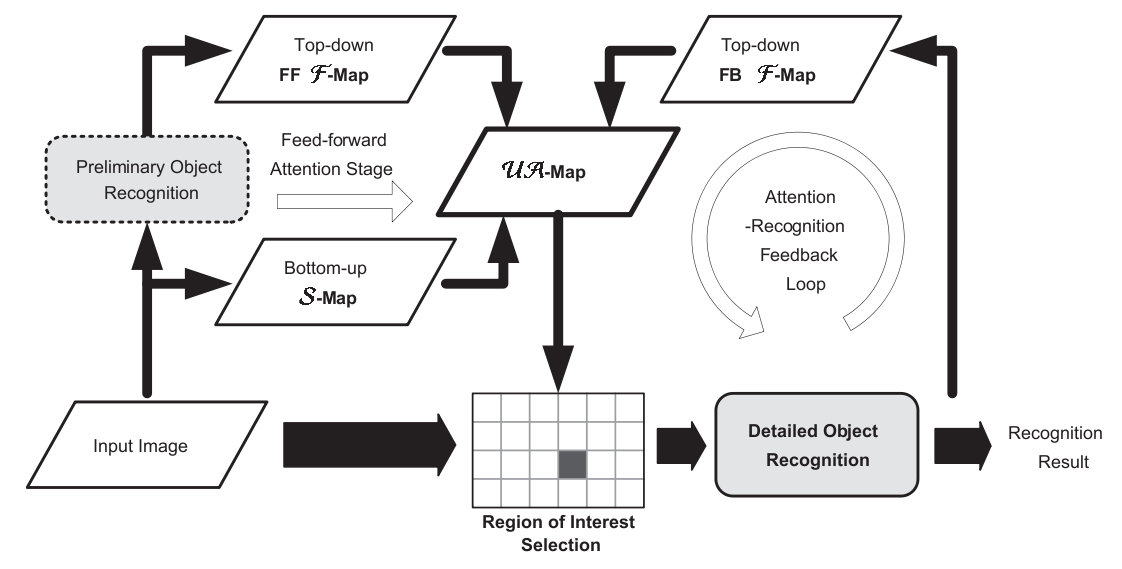
\includegraphics[scale=0.65]{alg.png}
	\caption{Fig.1: Outline of the UVAM algorithm.}
	\label{fig:1}
\end{center}


